%!TEX root = ../../../adrien_gomar_phd.tex

\subsection{Analysis of the convergence}
\label{sub:dream_ls_conv_coeff}

The convergence of the steady computation using the Roe~2 space scheme
is reported in Fig.~\ref{fig:dream_ls_convergence_roe2}. The residual
show a four order of magnitude decrease and the similarity
coefficients are convergence starting at 500~iterations.
Therefore, according to \citet{Casey2000}, the
solution is considered to be converged.
\begin{figure}[htb]
  \centering
  \subfigure[residuals]{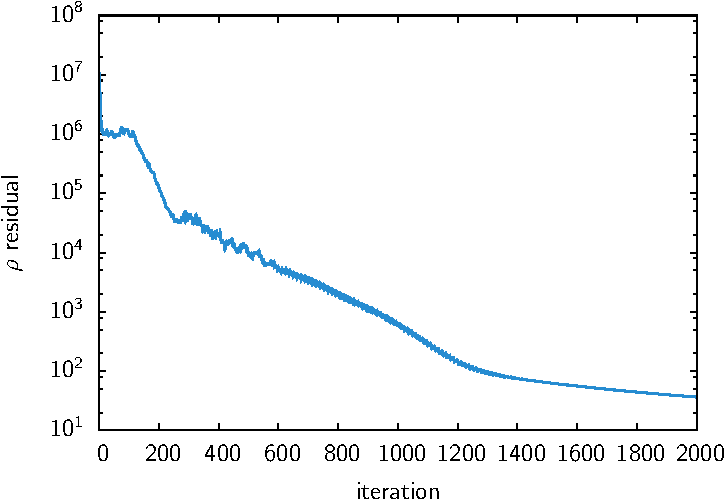
\includegraphics[width=.35\textwidth]{DREAM_LS_RESIDUALS_PPT.pdf}}
  \subfigure[$C_T$]{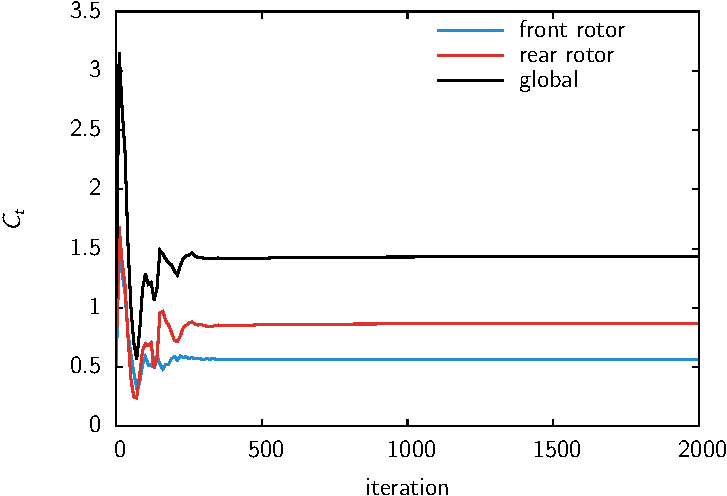
\includegraphics[width=.35\textwidth]{DREAM_LS_FORCES_CT_PPT.pdf}}
  \subfigure[$C_P$]{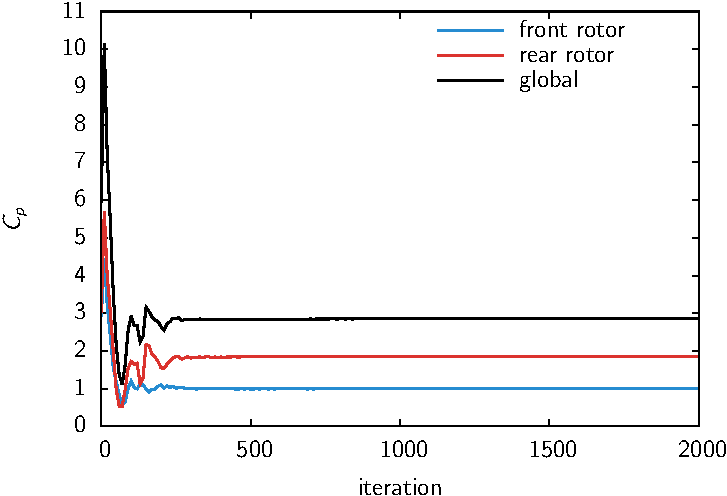
\includegraphics[width=.35\textwidth]{DREAM_LS_FORCES_CP_PPT.pdf}}
  \subfigure[$\eta$]{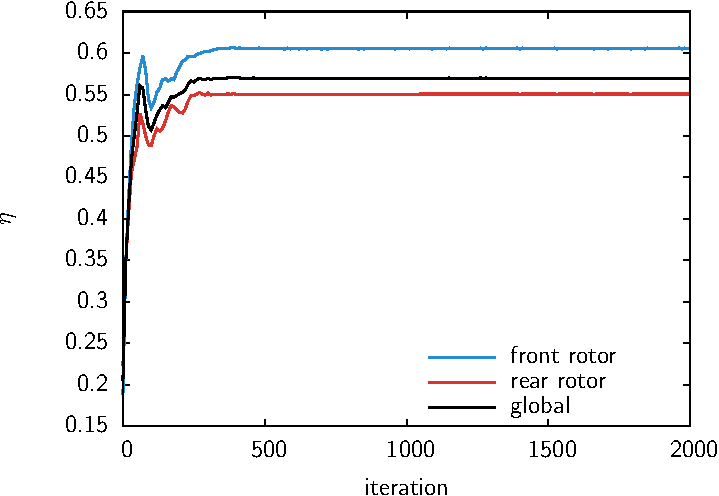
\includegraphics[width=.35\textwidth]{DREAM_LS_FORCES_ETA_PPT.pdf}}
  \caption{Low-speed isolated configuration: convergence of the steady
  computation.}
  \label{fig:dream_ls_convergence_roe2}
\end{figure}

\subsection{Radial profiles}
\label{sub:dream_ls_radial_profiles}

Six radial profiles are extracted,
positioned as shown in Fig.~\ref{fig:dream_ls_position_radial}
using Antares (see Appendix~\ref{app:antares}). The absolute
Mach number, absolute flow angle, static pressure, static
temperature, stagnation pressure and stagnation temperature
are shown in Fig.~\ref{fig:dream_ls_radial_profiles}
against the radial position expressed
relative to the radius of the front rotor blade.

The absolute Mach number, show in 
Fig.~\ref{fig:dream_ls_radial_profiles_ma}, is constantly increased through
the two rotors as it goes from the inflow condition value $M=0.2$
up to $M=0.4$. Note that above $R/h=1$, the Mach number
almost recovers the inflow condition. Moreover, it can be infer from the
$M_a$ evolution, that the stream tube is contracting.

The motivation for adding a second rotor to a propeller
was to recover the energy lost by the swirling flow
(recall Sec.~\ref{sub:cror_velocity_triangle}).
The absolute angle of the flow is shown in 
Fig.~\ref{fig:dream_ls_radial_profiles_alpha}. The front rotor
deviates the absolute velocity of almost $20^\circ$, justifying the need
for a second rotor. Between the fourth and the fifth extraction plane, namely
passing through the rear rotor, straighten the flow up. In fact,
the deflection angle is now close to $0^\circ$ for $0.3 \leq R/h \leq 0.7$.
Below that, the deflection angle remains negative. In the tip vortex region
of the rear rotor, one can the effect of the two tip vortices: between 
$0.8 \leq R/h \leq 0.9$, the front rotor tip vortex is seen as the 
deflection angle is positive, which is consistent with the positive
peak observe near the blade tip region in plane $P3$ and $P4$.

The goal of a CROR is to create thrust through an acceleration of 
the flow, not to produce static pressure as in a compressor stage.
This is highlighted in Fig.~\ref{fig:dream_ls_radial_profiles_ps}
where the evolution of the static pressure is shown.
In fact, the evolution of the static pressure lies with 2~\%
of its inflow value. A small increase is observed at each
rotor crossing. Upstream the rotors, the potential effects can
be seen. Actually, the flow is accelerated by the rotors, this acceleration
yielding a decrease of the static pressure 
(roughly through the Bernouilli theorem) and this pressure deficit is observed in
planes $P1$, $P2$ and $P4$.
\begin{figure}[htb]
  \centering
  \subfigure[position of the extraction planes]{
    \label{fig:dream_ls_position_radial}
    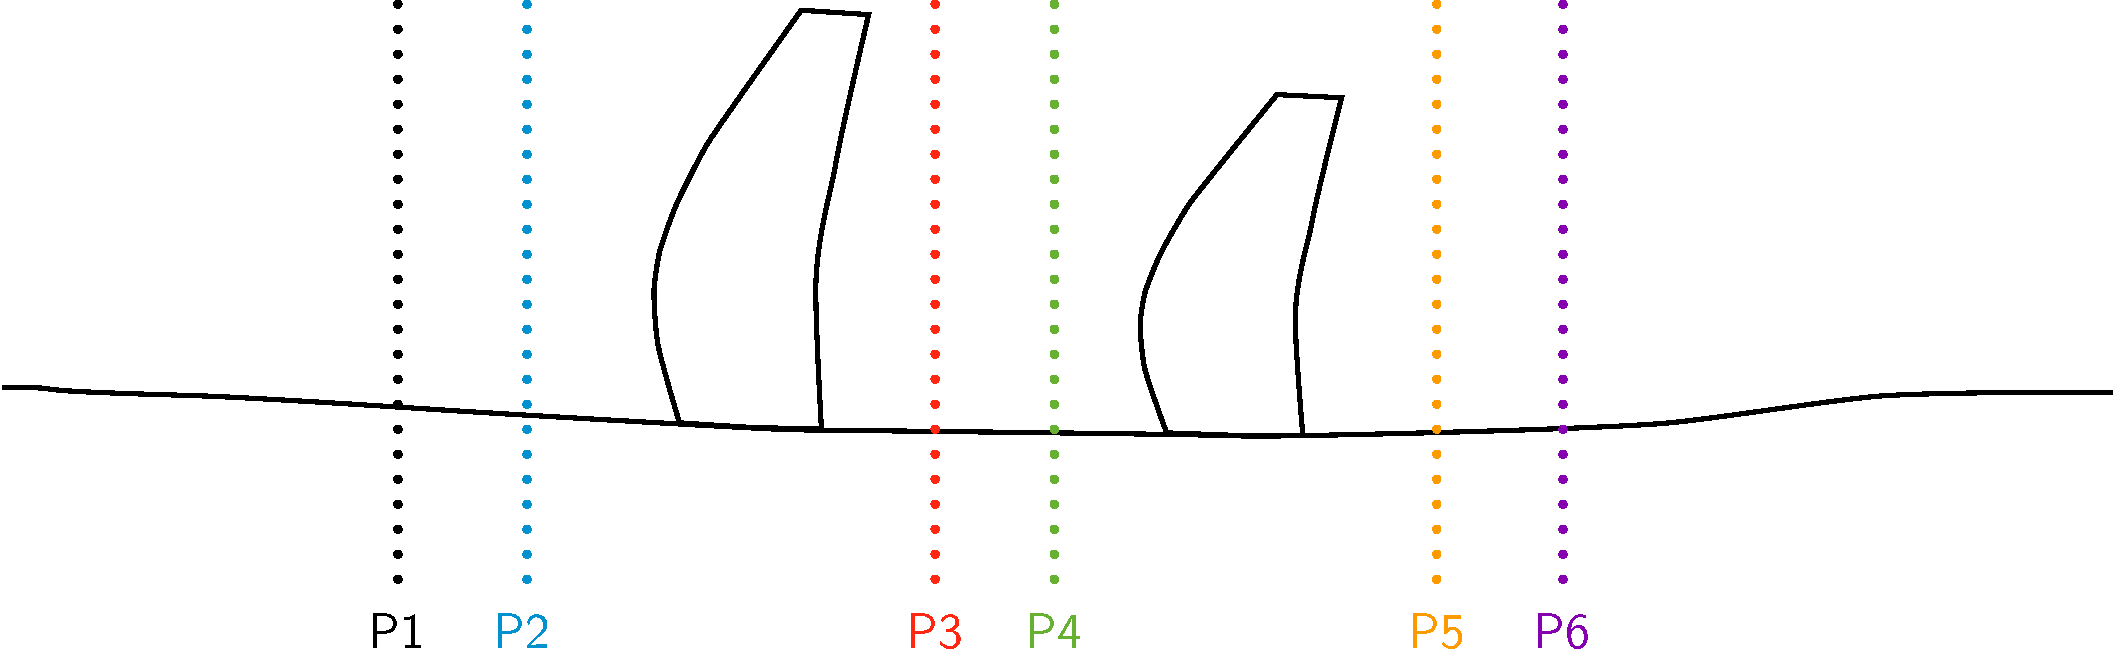
\includegraphics[width=.55\textwidth]{dream_position_azi_mean.pdf}}
  \subfigure[absolute Mach number]{
    \label{fig:dream_ls_radial_profiles_ma}
    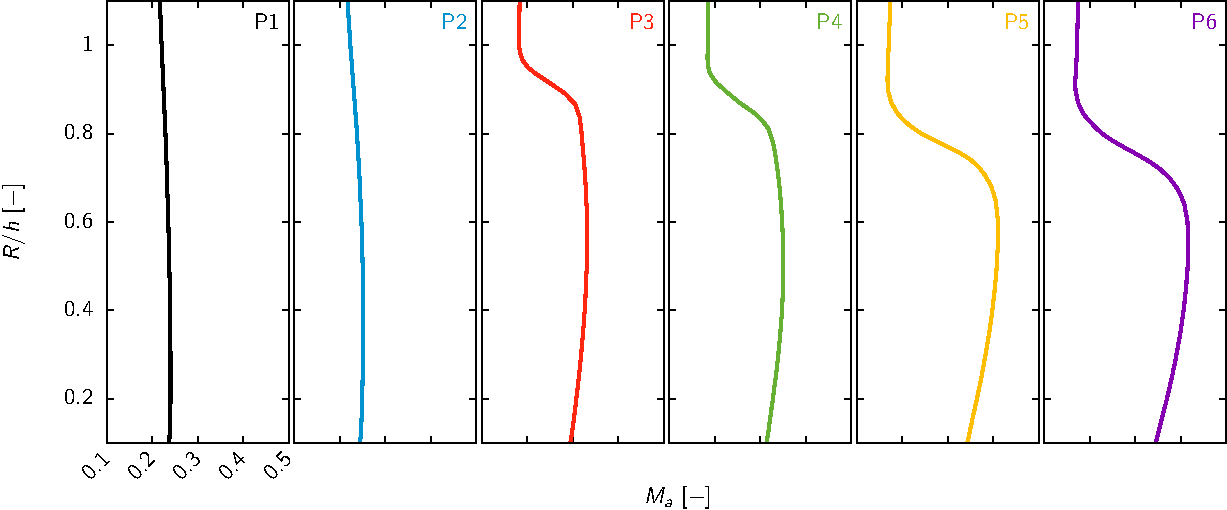
\includegraphics[width=.72\textwidth]{DREAM_LS_RANS_AZI_MEAN_PPT_macha.pdf}}
  \subfigure[absolution flow angle]{
    \label{fig:dream_ls_radial_profiles_alpha}
    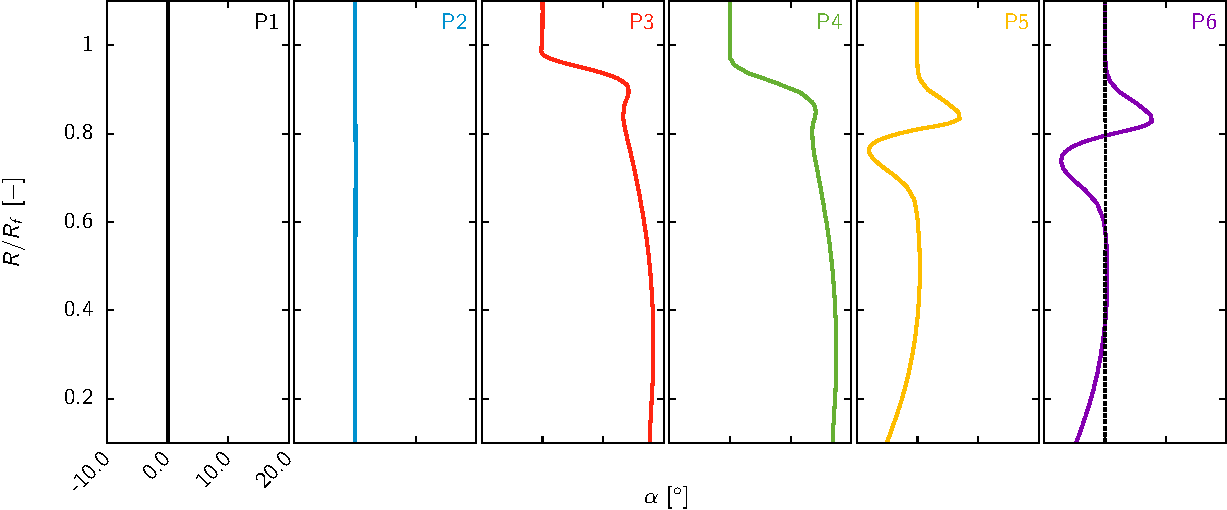
\includegraphics[width=.72\textwidth]{DREAM_LS_RANS_AZI_MEAN_PPT_alpha.pdf}}
  \subfigure[static pressure]{
    \label{fig:dream_ls_radial_profiles_ps}
    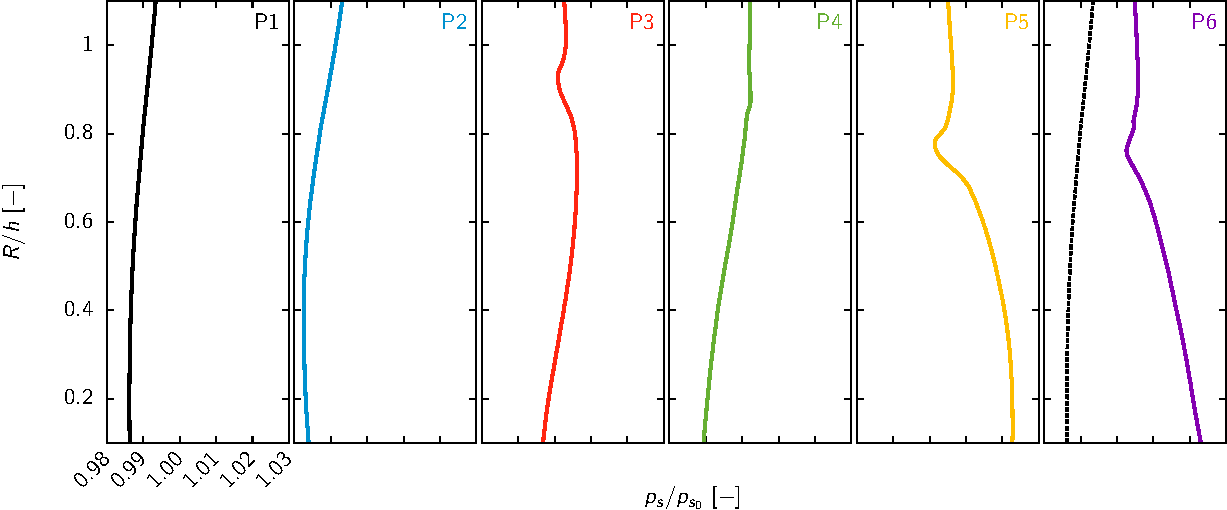
\includegraphics[width=.72\textwidth]{DREAM_LS_RANS_AZI_MEAN_PPT_ps.pdf}}
  \caption{Low-speed isolated configuration: radial profiles.}
\end{figure}
\setcounter{figure}{\value{figure}-1}
\begin{figure}[htb]
  \centering
  \setcounter{subfigure}{4}
  \subfigure[stagnation pressure]{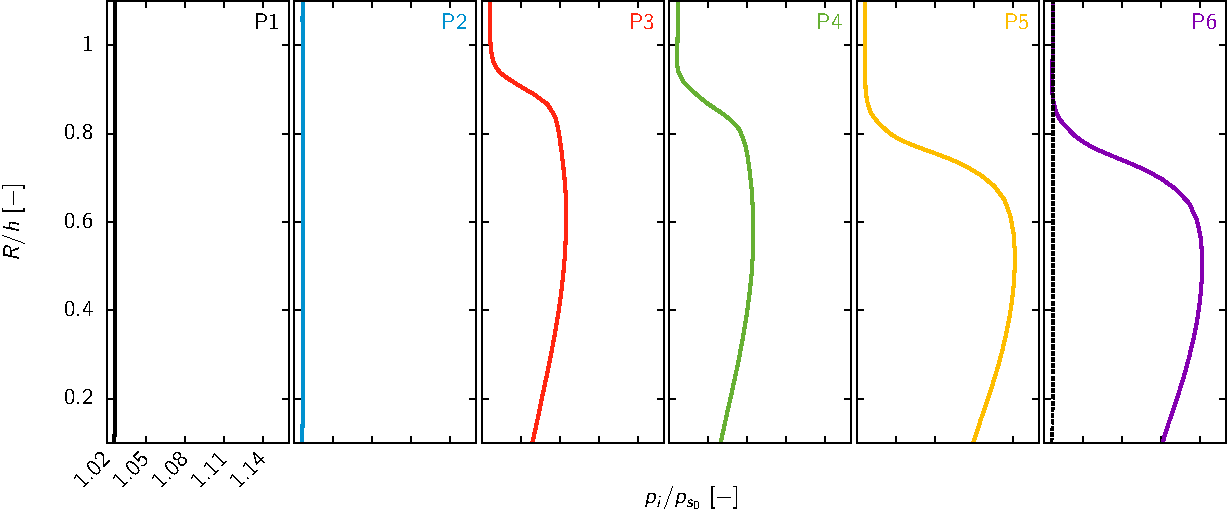
\includegraphics[width=.72\textwidth]{DREAM_LS_RANS_AZI_MEAN_PPT_pi.pdf}}
  \subfigure[stagnation temperature]{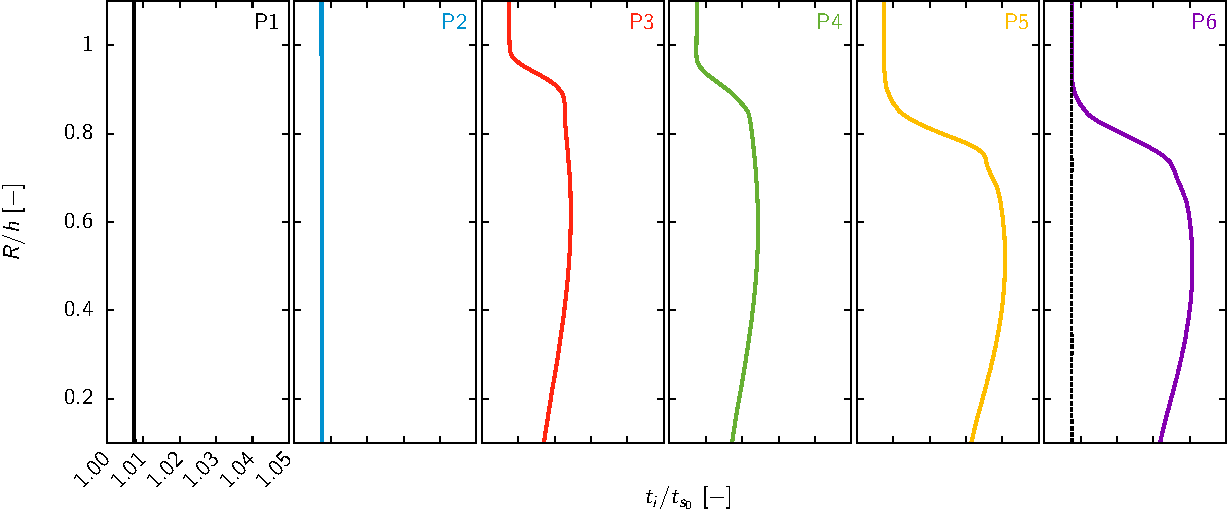
\includegraphics[width=.72\textwidth]{DREAM_LS_RANS_AZI_MEAN_PPT_ti.pdf}}
  \caption{Low-speed isolated configuration: radial profiles (contd.)}
  \label{fig:dream_ls_radial_profiles}
\end{figure}

\subsection{Flow field around the blades}
\label{sub:dream_ls_flow_field}

In this section, the local flow field is analyzed to
give some knowledge of the physic that develops in this
low-speed CROR configuration. This will help understand the
aeroelastic results obtained in Sec.~\ref{sec:dream_ls_ael_results}.




\begin{figure}[htbp]
 \centering
 \begin{tabular}{rccc}
   & $-k_p$ amont
   & $-k_p$ aval
   & Mach relatif\\
   \rotatebox{90}{\qquad\qquad 25~\%} 
   & 
   & 
   & 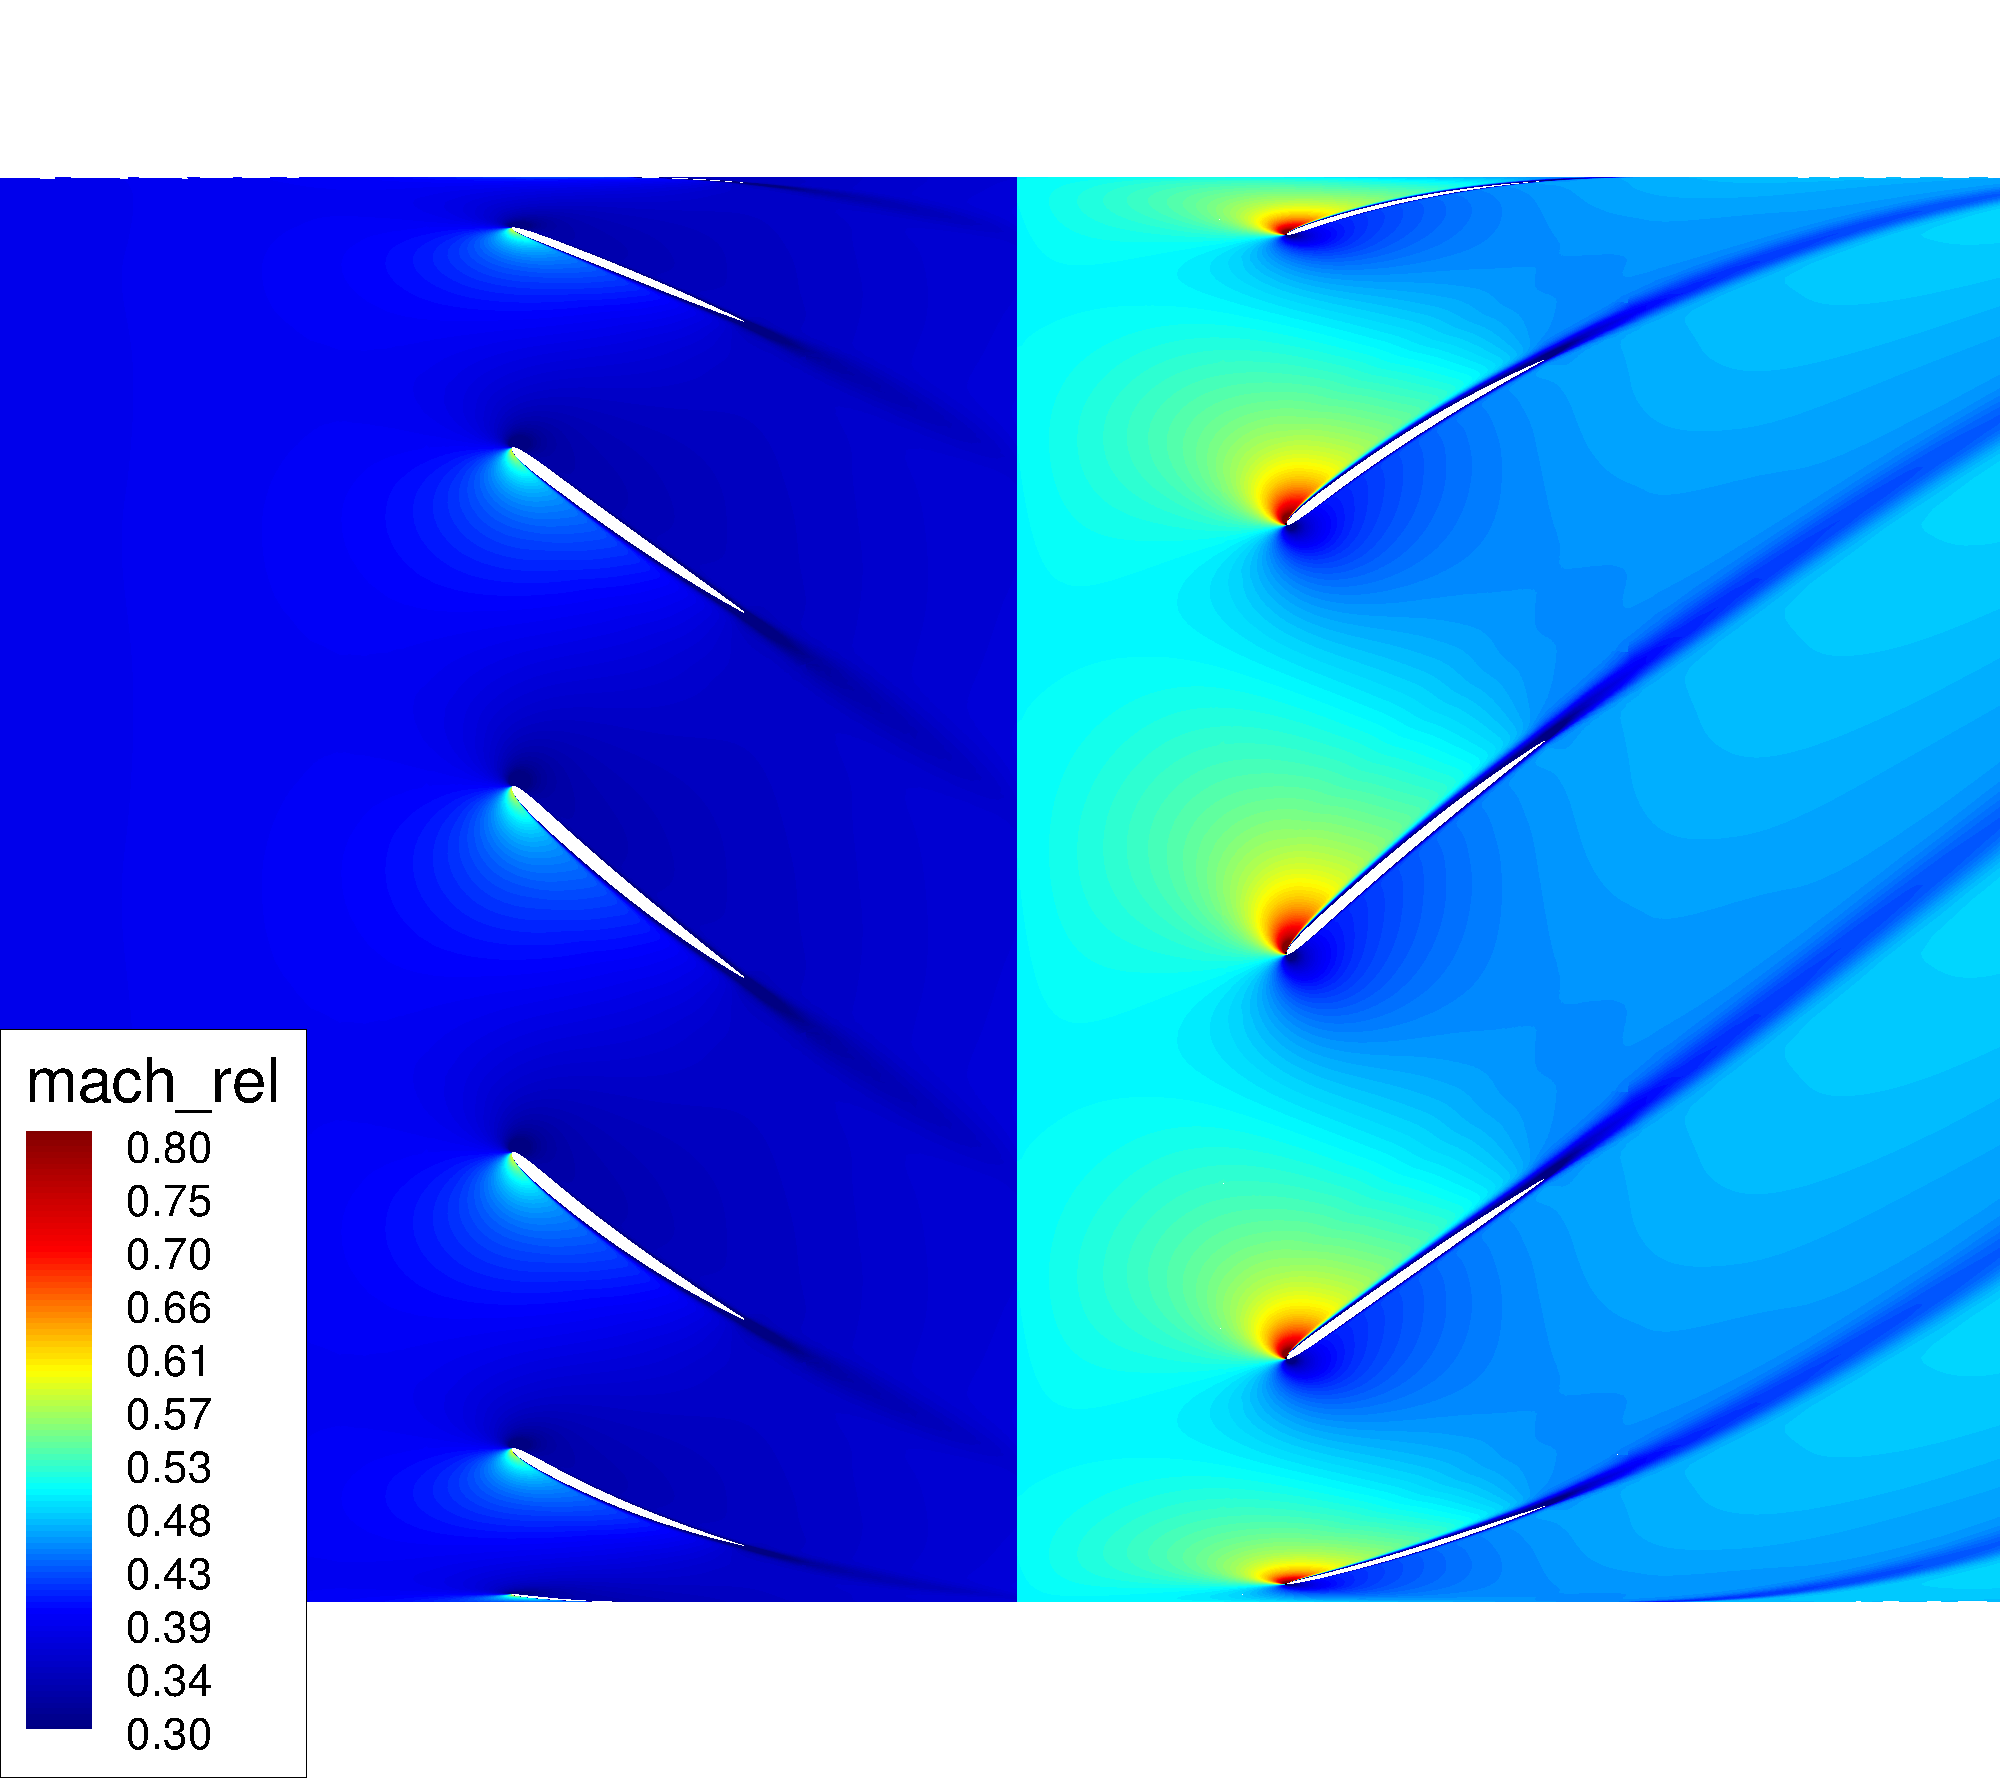
\includegraphics[width=0.28\textwidth]{DREAM_LS_RANS_roe2_sa_slice_r_25_mach_rel.png}\\
   \rotatebox{90}{\qquad\qquad 50~\%} 
   & 
   & 
   & 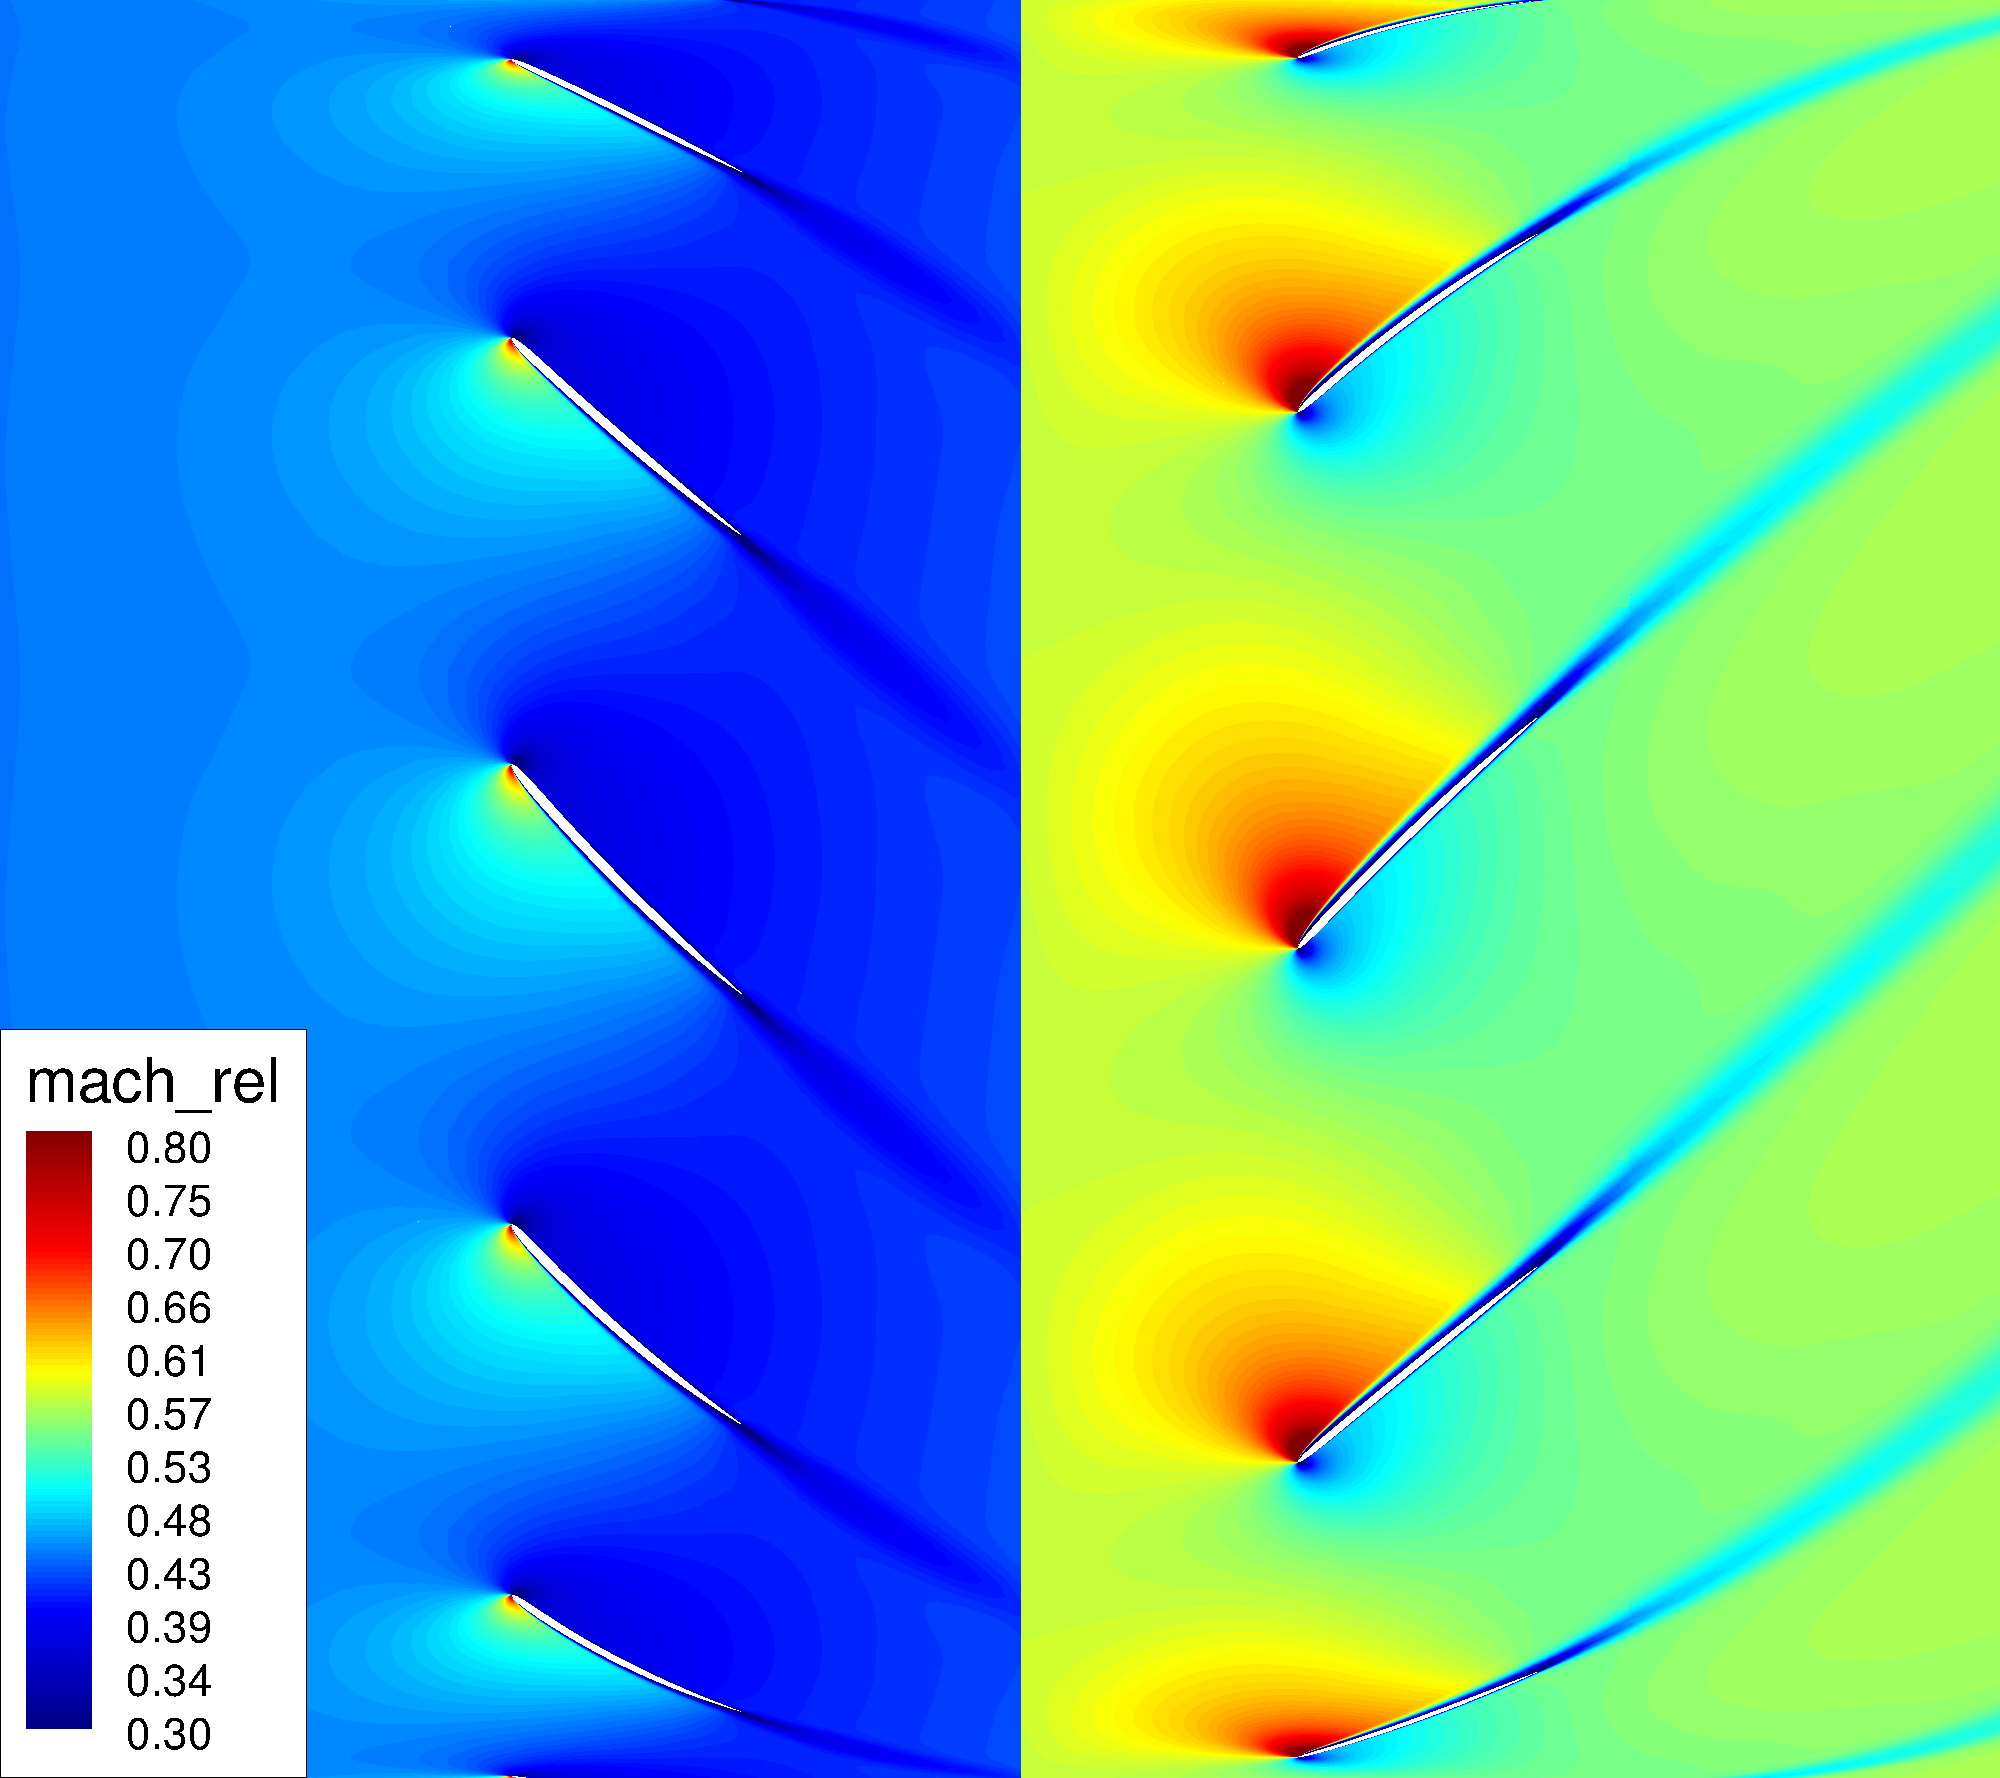
\includegraphics[width=0.28\textwidth]{DREAM_LS_RANS_roe2_sa_slice_r_50_mach_rel.png}\\
   \rotatebox{90}{\qquad\qquad 75~\%} 
   & 
   & 
   & 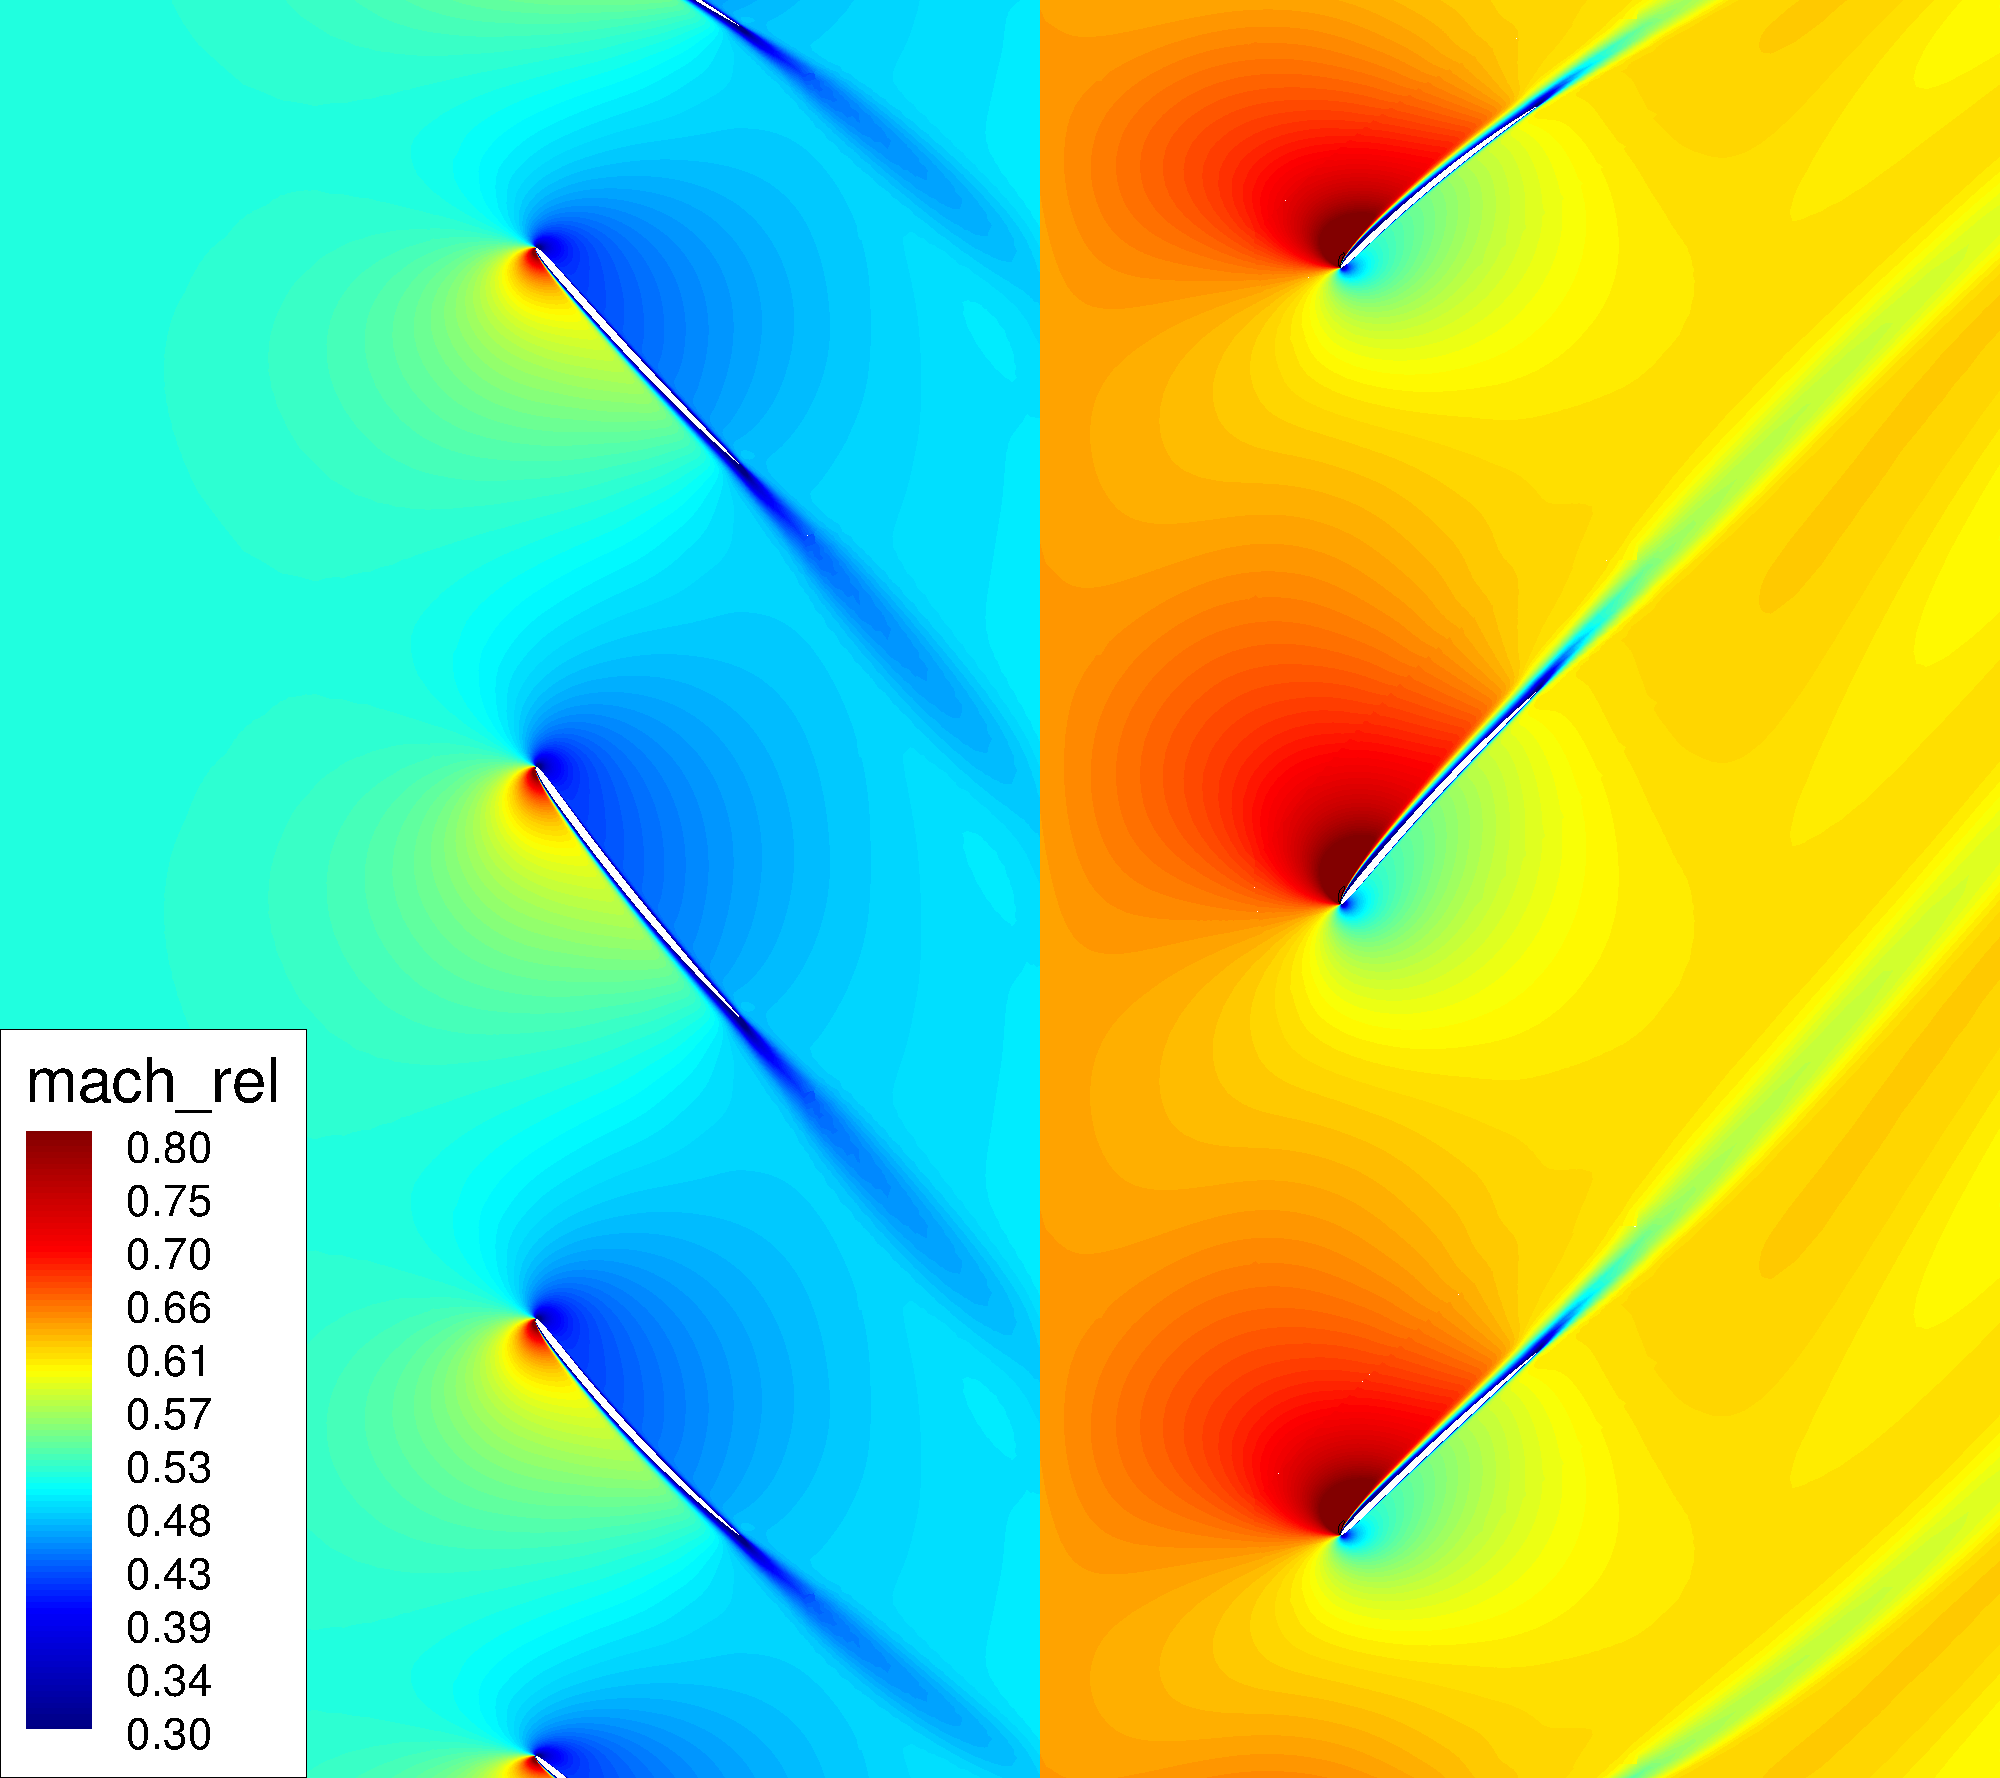
\includegraphics[width=0.28\textwidth]{DREAM_LS_RANS_roe2_sa_slice_r_75_mach_rel.png}\\
   \rotatebox{90}{\qquad\qquad 90~\%} 
   & 
   & 
   & 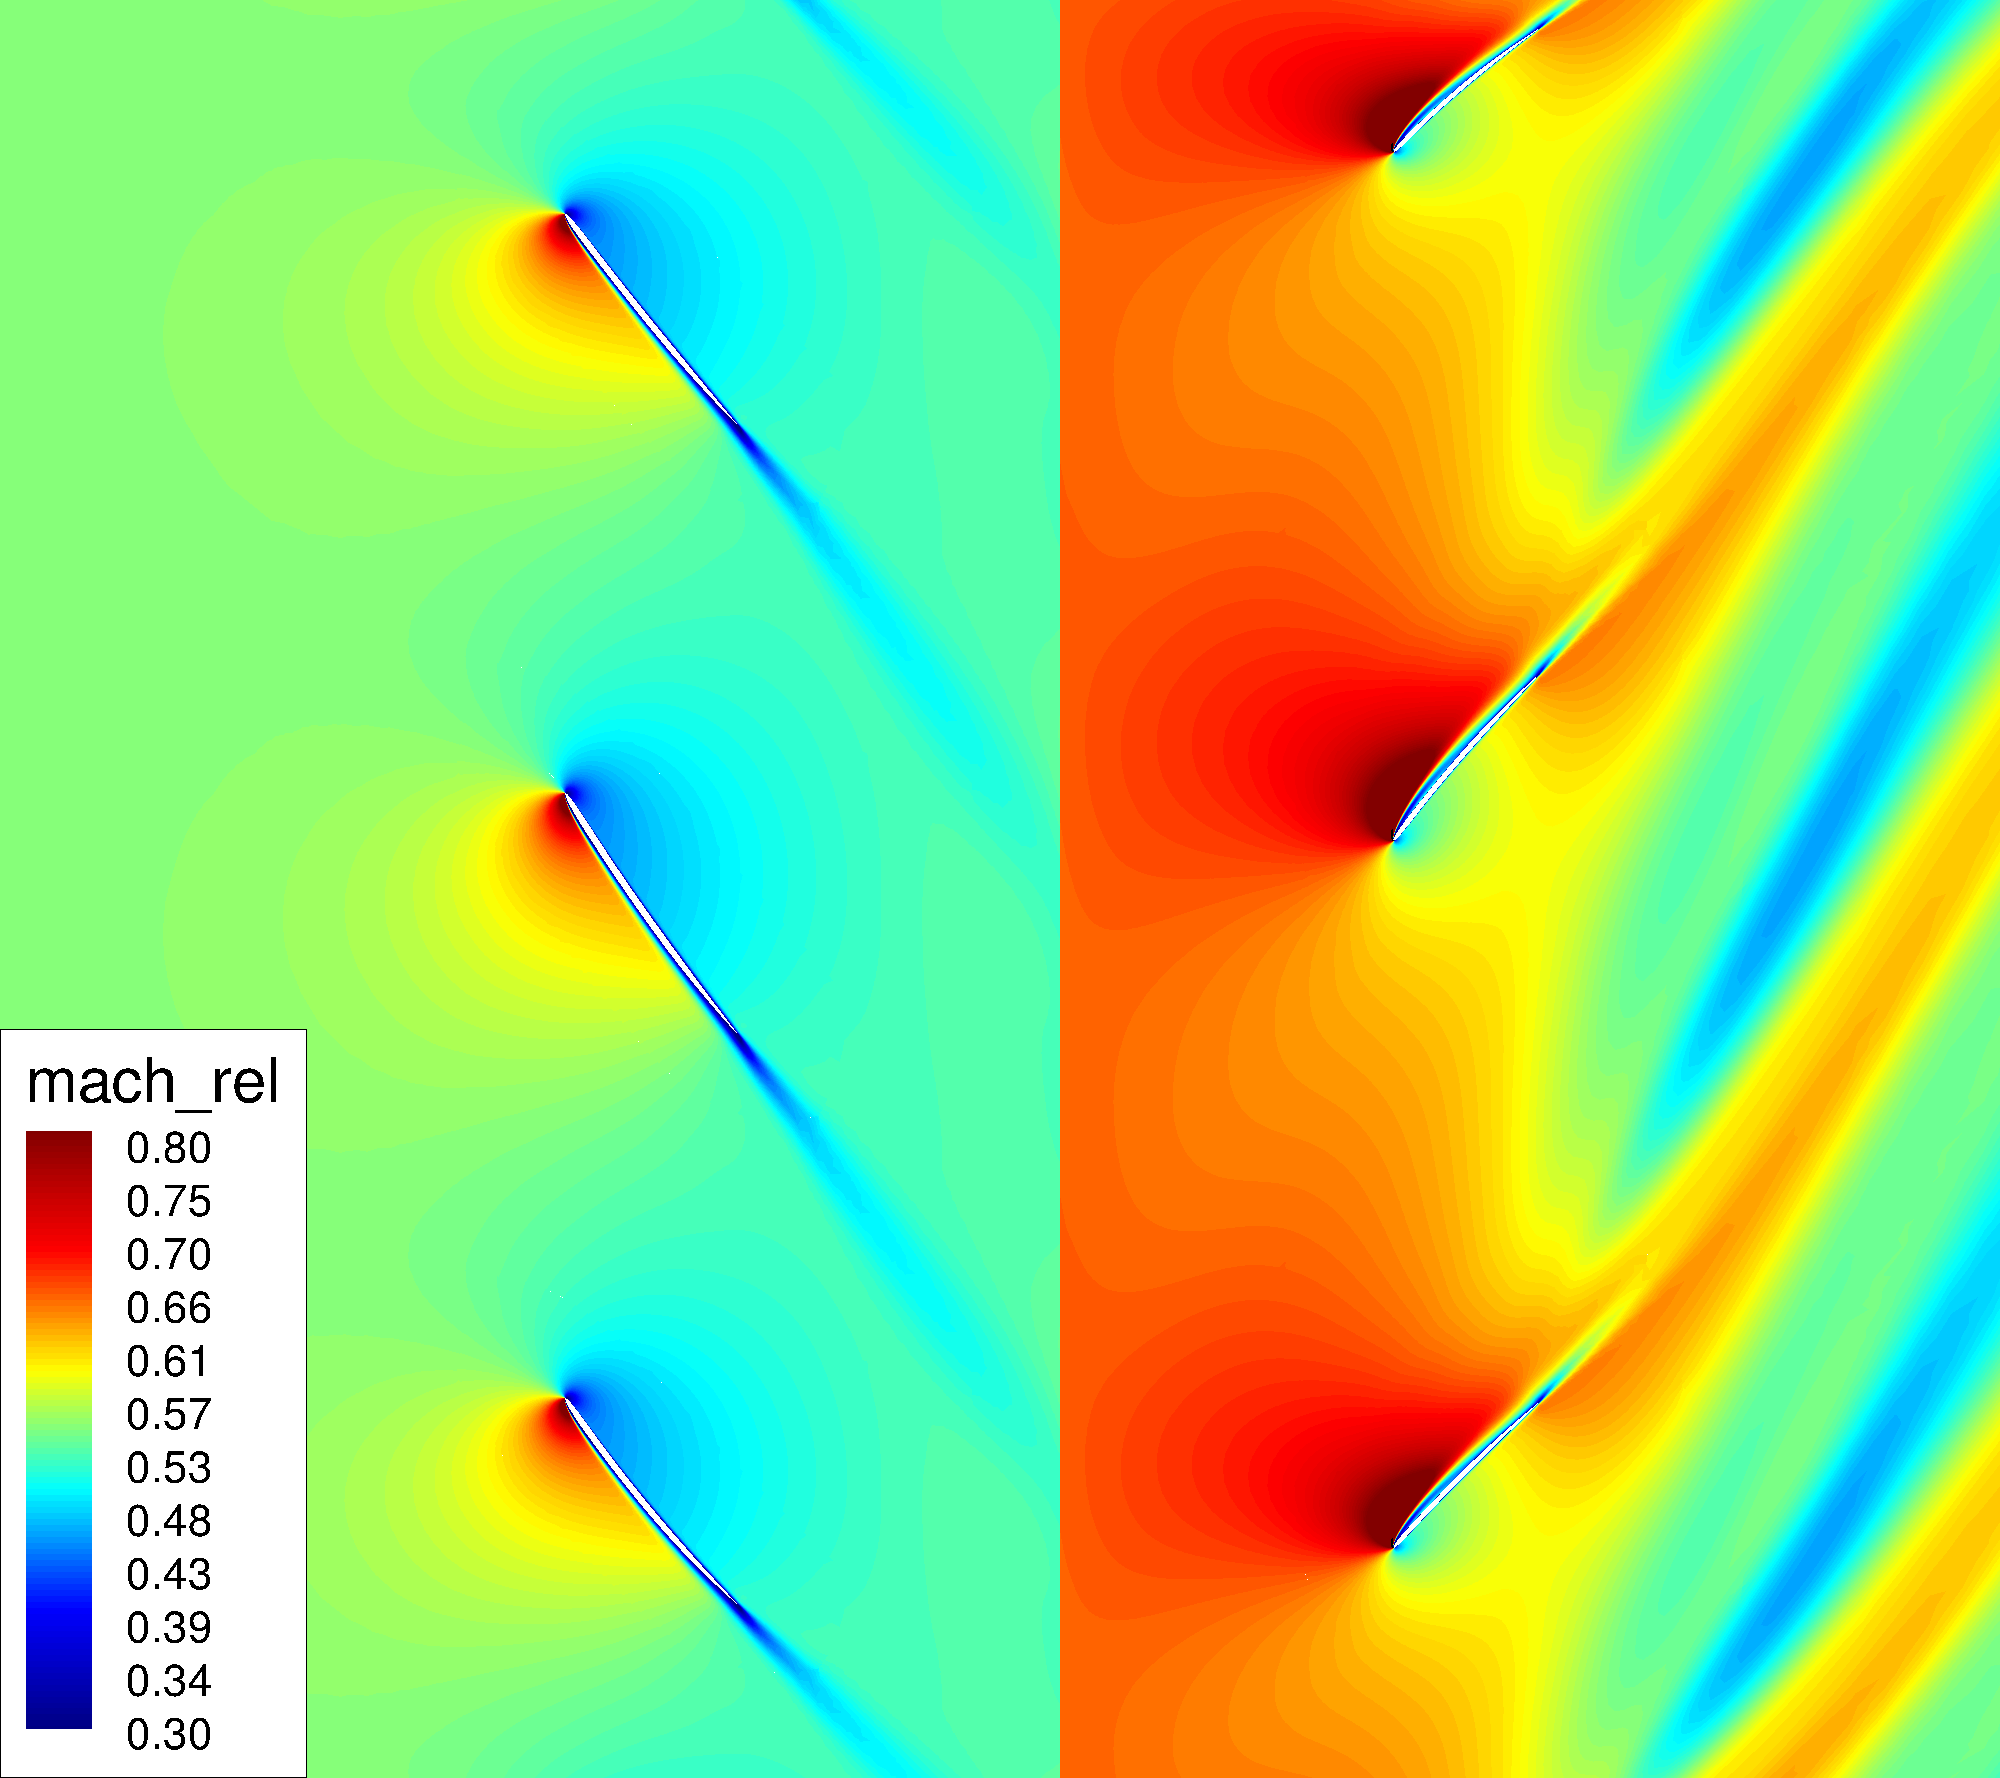
\includegraphics[width=0.28\textwidth]{DREAM_LS_RANS_roe2_sa_slice_r_90_mach_rel.png}\\
   \rotatebox{90}{\qquad\qquad 95~\%} 
   & 
   & 
   & 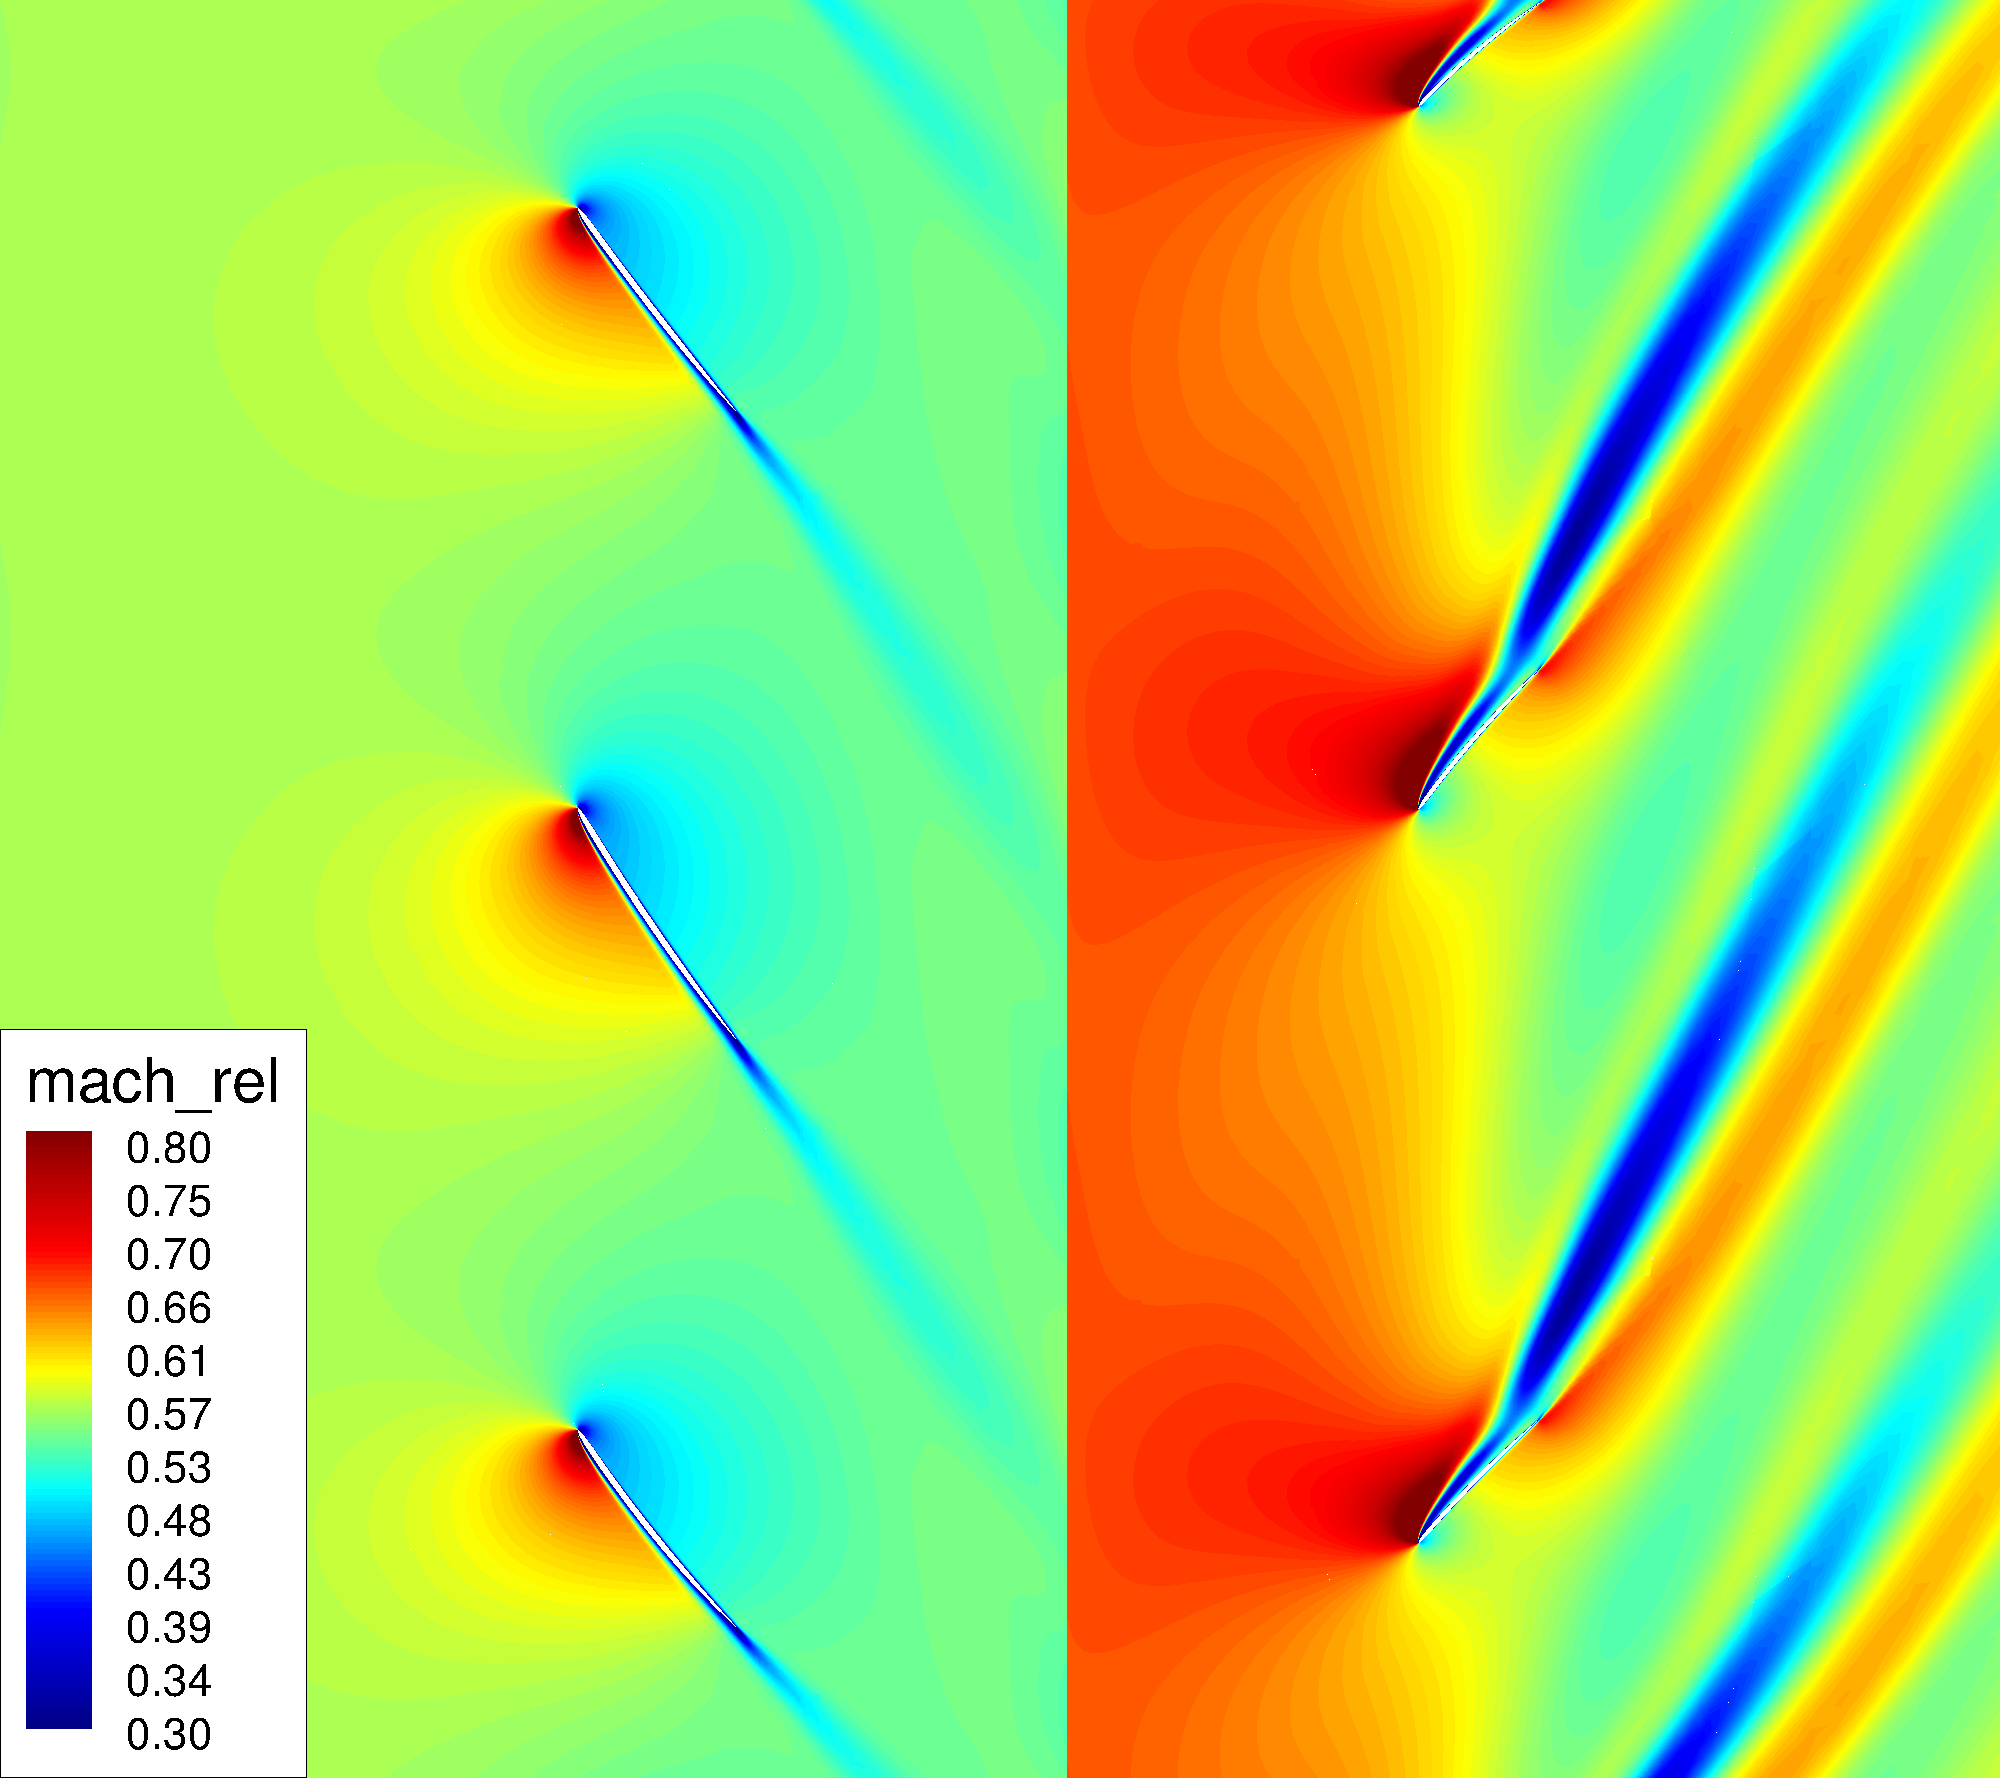
\includegraphics[width=0.28\textwidth]{DREAM_LS_RANS_roe2_sa_slice_r_95_mach_rel.png}  \end{tabular}
 \caption{$k_p$ et nombre de Mach relatif à différentes hauteurs de
   pales}
 \label{fig:kpmrel}
\end{figure}